\documentclass[11pt,a4paper]{article}
\usepackage[T1]{fontenc}
\usepackage[utf8]{inputenc}
\usepackage{lmodern,microtype}
\usepackage[a4paper,margin=19mm,headheight=15pt,headsep=7mm,footskip=10mm]{geometry}
\usepackage{array,tabularx,booktabs,enumitem,xcolor,graphicx,tikz,amsmath,fancyhdr}
\usetikzlibrary{arrows.meta,positioning}
\usepackage{xurl}
\usepackage[hidelinks]{hyperref}
\definecolor{ink}{RGB}{22,46,62}
\definecolor{light}{RGB}{237,243,246}
\hypersetup{pdftitle={AI-Based fraud detection for SEPA instant credit transfers: a technology risk assessment},pdfauthor={Codex analytical version prepared for Arici, Ferraboli and Brusamarello}}
\pagestyle{fancy}\fancyhf{}
\fancyhead[L]{\small Technology Risk Governance | Major assignment}
\fancyhead[R]{\small 25 November 2026}
\fancyfoot[L]{\scriptsize Codex analytical version | GenAI disclosure on page 15}
\fancyfoot[R]{\small\thepage/15}
\setlength{\parindent}{0pt}\setlength{\parskip}{6pt}
\setlist[itemize]{nosep,leftmargin=16pt,topsep=3pt}
\setlist[enumerate]{nosep,leftmargin=18pt,topsep=3pt}
\renewcommand{\arraystretch}{1.17}
\newcolumntype{Y}{>{\raggedright\arraybackslash}X}
\newcolumntype{P}[1]{>{\raggedright\arraybackslash}p{#1}}
\newcommand{\heading}[2]{\vspace*{1mm}{\small\color{ink}\textbf{#1}}\par\vspace{2mm}{\LARGE\color{ink}\textbf{#2}}\par\vspace{3mm}}
\newcommand{\sub}[1]{\par\vspace{2mm}\textbf{\color{ink}#1}\par}
\newcommand{\src}[1]{{\small[#1]}}
\newcommand{\newpageof}[2]{\clearpage\normalsize\fontsize{10.5}{12.5}\selectfont\heading{#1}{#2}}
\newcommand{\risk}[2]{\sub{#1. #2}}
\begin{document}
\fontsize{10.5}{12.5}\selectfont
\heading{Approved topic | Technology risk assessment}{AI-Based fraud detection for SEPA instant credit transfers: a technology risk assessment}
\vspace{2mm}
\textbf{Group}\par
Michele Attilio Arici --- \href{mailto:micheleattilio.arici@mail.polimi.it}{micheleattilio.arici@mail.polimi.it}\\
Andrea Ferraboli --- \href{mailto:andrea.ferraboli@mail.polimi.it}{andrea.ferraboli@mail.polimi.it}\\
Michelangelo Brusamarello --- \href{mailto:michelangelo.brusamarello@mail.polimi.it}{michelangelo.brusamarello@mail.polimi.it}
\sub{Executive assessment}
This preliminary assessment examines a retail bank's adoption of an AI system that screens outgoing SEPA instant credit transfers before execution. The objective is to reduce fraud loss while preserving payment speed and limiting rejection of legitimate payments. The bank is an analytical reference organisation; no institution, dataset or vendor performance is represented as observed.

AI may identify suspicious combinations that static rules miss, but can also add false rejections, operational dependencies and an additional attack surface. A model's predictive score is therefore insufficient evidence for adoption. The decision concerns the entire payment service: data, decision policy, authorisation, technical execution, customer response and ongoing governance.

The assessment uses preliminary hazard analysis (PHA) to examine twelve scenarios. It evaluates consequences, dependencies and evidence gaps, linking each scenario to controls, accountable roles and a specific treatment decision. It deliberately avoids numerical likelihoods and composite risk scores unsupported by bank data. The central finding is that controls can make a bounded evaluation defensible, while public evidence cannot establish that production risk is acceptable for a particular bank.

\textbf{Recommendation:} retain the existing controlled service and progress only to an authorised shadow evaluation, followed by a restricted pilot if legal, operational and performance gates are met. Unconditional production adoption is not supported. This is the conclusion of the present analysis; no bank implementation or authorisation is asserted.
\sub{Scope of the conclusion and reading guide}
The approved topic is assessed as an adoption decision, not a comparison of algorithms in isolation. PHA is selected because the architecture is preliminary, frequency data are unavailable and the main conflicts cross technical, human and organisational boundaries. The question is which deployment conditions are defensible, rather than whether an unspecified AI model is accurate. This is a Codex-authored analytical version prepared for the group; actual AI contributions, the course-policy constraint and signature status are stated on p.~15.

Pages 2--4 define the business case, system and evidence. Pages 5--10 cover identification, analysis and evaluation. Pages 11--13 address treatment, sensitivity and the adoption decision. References and disclosure complete the report. Evidence files preserve fuller source locations and limitations.

\newpageof{1 | Business case}{Adoption options and value at risk}
\sub{Service context and loss mechanisms}
Instant transfers are a continuously available retail payment service. A payer may be deceived into authorising a transfer, or an attacker may act through compromised credentials or a compromised session. A valid authentication and a matching payee name do not establish that the payer's economic intention is legitimate. Once the payment is executed, recovery can be difficult and is not a substitute for prevention. \src{P01, P02, P07, P08}

The business case concerns the \emph{incremental} effect of AI relative to a competent existing fraud-control baseline, including applicable authentication, transaction monitoring and verification of payee (VoP). It does not compare AI with an unprotected bank. Benefits include avoided unrecovered losses and reduced unnecessary interventions; costs include false rejection, customer remediation, validation, infrastructure, investigation and operational disruption. The allocation of losses between bank and customer affects private incentives, but both remain relevant to the service objective.
\sub{Alternatives and selected adoption path}
\par{\small\begin{tabularx}{\textwidth}{@{}P{25mm}YY@{}}\toprule
Option & Expected contribution & Main trade-off and decision evidence\\\midrule
A. Retain rules & Known operating process; strengthen current controls and data. & Adapting to new fraud patterns may require manual rule changes. Provides the comparator for every experiment.\\
B. AI in shadow & Score the same requests without controlling execution. & Tests data quality and timing; cannot directly prove counterfactual losses avoided by blocking. Preferred first evaluation stage.\\
C. AI plus rules & Model informs a bounded, versioned decision policy with independent safeguards. & Potential better detection; adds latency, model risk and intervention costs. Conditional pilot candidate.\\
D. Broad automatic rejection & AI-led blocking across the eligible portfolio. & Largest exposure to error, legal and availability consequences. Not justified by available evidence.\\\bottomrule
\end{tabularx}\par}
\sub{Implementation concept}
The reference solution is a supervised tabular classifier, for example a gradient-boosted model, trained on properly matured fraud outcomes. This is a design assumption rather than a selected vendor, algorithm or claimed result. It returns a score and supporting reason codes. A separate policy engine combines this output with rules, data-quality flags and service-state information. No generative model is required to decide whether to execute a payment.

Build and buy alternatives share the same assurance obligations. An internal build increases control of features and retraining but requires specialist capacity. A vendor service may accelerate implementation while creating data, audit, concentration and exit dependencies. The bank retains accountability. \src{P05}
\sub{Decision rule for adoption}
Value is demonstrated only if incremental fraud benefit exceeds incremental friction and lifecycle cost within binding constraints. Lower average fraud loss cannot compensate for an unlawful decision process or an unsafe execution state. A quantitative net benefit cannot be estimated without bank-specific exposure, label maturity, customer impact and cost data. Page 12 specifies the required comparison without filling gaps with invented figures.

\newpageof{2 | System description}{Boundary, payment flow and responsibilities}
\begin{center}
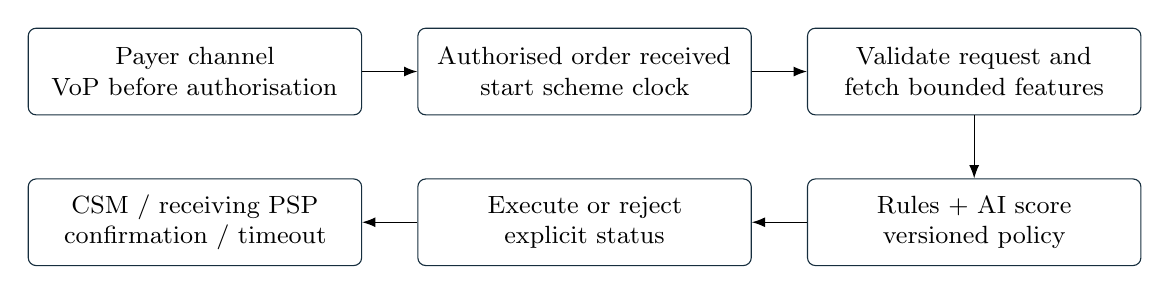
\begin{tikzpicture}[node distance=4mm,>=Latex,every node/.style={font=\small},box/.style={draw=ink,rounded corners=1mm,align=center,text width=40mm,minimum height=11mm}]
\node[box](a){Payer channel\\VoP before authorisation};
\node[box,right=7mm of a](b){Authorised order received\\start scheme clock};
\node[box,right=7mm of b](c){Validate request and\\fetch bounded features};
\node[box,below=8mm of c](d){Rules + AI score\\versioned policy};
\node[box,left=7mm of d](e){Execute or reject\\explicit status};
\node[box,left=7mm of e](f){CSM / receiving PSP\\confirmation / timeout};
\draw[->](a)--(b);\draw[->](b)--(c);\draw[->](c)--(d);\draw[->](d)--(e);\draw[->](e)--(f);
\end{tikzpicture}
\end{center}
{\small Figure 1. Reference architecture used in the assessment. Simplified sequence; bank-specific VoP, authentication and funds checks require implementation validation. No serial online analyst queue is assumed.}
\sub{Timing and decision semantics}
The statutory execution window starts at receipt of the payment order, not after completion of AI scoring. The current EPC rulebook is the 2025 SCT Inst rulebook v1.2, effective 30 September 2026; its operational sequence includes 5/7/9-second sub-timelines within the regulatory ten-second limit. Ten seconds is not an AI-processing allowance. The system must measure the entire request path and reserve time for downstream execution and confirmation. \src{P01, P02}

The decision policy returns a definite outcome within the available budget; rejection requires a valid contractual/legal basis, including refusal of an order under PSD2 Article 79, distinct from blocking a payment instrument under Article 68. It is not an unlimited model discretion. \src{P10} Additional customer interaction is not assumed to pause the clock. If more investigation is needed, the order must follow a legally valid, explicitly defined outcome and any later instruction must be a new authorised request. On timeout or uncertain settlement, the system reconciles status and applies required restoration and notification rules; it never silently resubmits an uncertain payment.
\sub{Boundary and dependencies}
For legal applicability, assume an EU retail credit institution established in the euro area. This is a declared analytical assumption; SEPA membership alone does not establish EU regulatory scope. Inside: channel integration, point-in-time features, score service, policy engine, payment interface, logs, model deployment, monitoring and fallback. External dependencies: core banking, identity/authentication, VoP service, clearing and settlement mechanism (CSM), receiving PSP, cloud/vendor and telecommunications. Fraudsters and customers interact with the boundary. Sanctions and AML remain separate obligations and controls; this report does not redesign them.

Data include amount, beneficiary identifier, transaction history, device/session signals where lawful, and subsequent fraud outcomes. Exclude features unavailable at the decision instant. Separate training and production access; minimise and protect identifiers, define retention, and preserve provenance. Labels arrive after the payment and can be incomplete or selectively observed. \src{P06, P09}
\sub{Accountability assumptions}
The payments owner owns service outcomes and timing; fraud operations owns intervention policy; the model owner owns training and monitoring; independent validation challenges the model. IT operations owns restoration and reconciliation, the CISO owns security assurance, procurement owns supplier evidence, and the DPO/legal function assesses processing and decision rights. A risk committee or delegated accountable executive accepts residual risk. These responsibilities specify the operating model required by this analysis; they are not observations about a named bank.

\newpageof{3 | Reference documentation}{Evidence base and course alignment}
\sub{Search and selection}
Research was conducted on 25 November 2026. Queries targeted SCT Inst timing and current rulebook, EU payment fraud, financial-fraud AI classification, operational resilience, privacy, authentication, and realistic fraud-model evaluation. Official EPC, ECB/EBA, EUR-Lex and Commission sources were prioritised. An original peer-reviewed fraud-modelling study was selected to explain methodological pitfalls, not to supply SEPA performance estimates. No vendor accuracy claim is used to infer benefit.

Candidate documents were screened for primary authorship, explicit scope, current version, access to substantive text and relevance to one of the twelve scenarios. Downloaded files were reopened and checked. The machine-readable register records original URL, date, local path or retrieval limitation, relevant locations, supported claims and evidence quality. Search and retrieval logs distinguish full documents from official explanatory pages and inaccessible downloads. JEV and Firecrawl tools were not exposed in this session; web search and direct lawful retrieval were used instead.
\sub{What the evidence supports}
The EBA/ECB 2025 report provides EEA payment-fraud context for 2022--2024. It reports EUR 2.5 billion in fraudulent credit-transfer value in 2024, distinct from EUR 2.200 billion in credit-transfer losses. These are different measures with potentially different reporting periods. Its instant-transfer box has incomplete country coverage and identifies Italian submissions under revision. Neither aggregate measure establishes this bank's instant-transfer fraud probability or AI effectiveness. \src{P08, pp.~6, 10, 13--14, 34--35}

The scientific study addresses realistic fraud-detection evaluation, including imbalance, changing patterns and delayed verification. Its card-payment setting supports a warning about evaluation design, not transfer of reported performance to SEPA. \src{P09} Legal and scheme sources define applicable constraints; they do not establish that the proposed controls work in a particular bank.
\sub{Concepts applied from the course}
\par{\small\begin{tabularx}{\textwidth}{@{}P{38mm}YP{20mm}@{}}\toprule
Course source, PDF page & Application in this assessment & Report\\\midrule
Class 1--2, pp.~29--35 & Risk as uncertainty affecting objectives; hazard, vulnerability and event distinguished; barriers. & 1--3, 7--10\\
SSE Class 3, pp.~13, 29--33, 43 & Context and criteria before evaluation; preliminary qualitative analysis; proportional treatment. & 5--6\\
SSE Classes 3--4, pp.~47--53 / 6--9, 27 & Compare FMEA, FTA and ETA with PHA; avoid unsupported quantification. & 5, 9\\
Cyber governance 2026--27, pp.~20, 42--43, 48, 53 & Appetite, organisational vulnerabilities, treatment and risk register. & 6--11\\
IT Risk Management, pp.~15--18, 33--34 & Objectives to process/assets; controls, coverage and residual risk. & 7--13\\
HOF Class 7; HRO pp.~9, 13 & Latent conditions, active errors, expertise and recovery capability. & 10--11\\\bottomrule
\end{tabularx}\par}
{\small Full filenames and finer references are in the course evidence map. PDF page numbers are used; they may differ from printed slide numbers. English is an operational choice, not an explicit language requirement.\par}

\newpageof{4 | Assessment method}{Why PHA is the selected method}
\sub{Selection and justification}
This assessment adopts course-taught preliminary hazard analysis (PHA), organised through the ISO 31000 stages of identification, analysis and evaluation and documented in a scenario register. PHA matches the concept/design stage and the secondary evidence available. It can examine fraud that passes a technically functioning system as well as component failure and organisational conditions. The alternatives below were compared against scope, data needs and ability to inform adoption. \src{course assignment pp.~5--7; SSE Class 3 pp.~13, 29--33}
\par{\small\begin{tabularx}{\textwidth}{@{}P{27mm}YY@{}}\toprule
Candidate & Fit to available information & Limitation / proposed use\\\midrule
PHA / scenario register & Early design, secondary evidence, heterogeneous technical and organisational causes. & Coarse and judgement-dependent; document causation, uncertainty and control evidence. Selected primary method.\\
FMEA / FMECA & Component functions, failure modes and effects; valuable for integration design. & Component detail unavailable; deceptive but technically valid payments can occur without component failure. No unsupported RPN.\\
FTA & Deductive causes of a defined top event, useful for timeout or unsafe release. & Numerical propagation requires credible basic-event data and dependencies. Qualitative reasoning only here.\\
ETA & Sequence of barrier success/failure after an initiating event. & Branch probabilities unavailable; useful for discussing fallback consequences, not for loss estimates.\\
Quantitative loss model & Direct business comparison when exposure, losses and intervention costs are known. & Public aggregates cannot calibrate the bank. Use symbolic sensitivity on p.~12, not simulation.\\\bottomrule
\end{tabularx}\par}
\sub{Application and limits}
\textbf{Context:} define objectives, boundary, stakeholders and decision criteria (pp.~1--3, 6). \textbf{Identification:} identify threat or initiating condition, vulnerability, event and consequence across lifecycle stages (p.~7). \textbf{Analysis:} examine cause, existing baseline, proposed barriers, dependencies and uncertainty (pp.~8--10). \textbf{Evaluation:} compare each configuration with criteria and distinguish design rejection, shadow evaluation and conditional pilot requirements (pp.~6--10). \textbf{Treatment and review:} assign ownership, evidence and monitoring requirements (pp.~11--13).

Consequences are analysed by affected objective, potential scale and reversibility. Payment-integrity and rights-critical defects cannot be offset by business benefit. Fraud loss, legitimate-payment harm and disruption are assessed separately, including escalation at scale. Bank frequency remains unestimated. Legal/timing constraints are directly documented; R2--R3 use transferable card-fraud research; other causal scenarios are design inferences grounded in the course. Evidence strength is not a likelihood score.

This is a preliminary design assessment, not a calibrated enterprise risk ranking. A severe scenario with unresolved likelihood is not described as low risk. ALARP informs proportionate further treatment and explicit acceptance, but industrial safety boundaries are not imported as banking risk limits. \src{SSE Class 3 p.~43}

\newpageof{5 | Evaluation criteria}{Acceptability is constrained by evidence}
\sub{Decision rules applied to configurations}
\textbf{Reject the design} where it resets the payment clock, creates duplicate/ambiguous execution, uses unbounded fallback or processes data unlawfully. \textbf{Support isolated shadow evaluation} where lawful data use and operational separation are established: scoring adds no customer decision risk, but still requires capacity and security controls. \textbf{Permit a live pilot only conditionally} on the scenario-specific evidence below, bounded exposure and accountable acceptance. No test is represented as already passed.

Treatment has three evidence priorities: \textbf{P}, design prerequisites for live decisions (R5--R8, R11); \textbf{V}, validation of benefit and customer harm (R1--R4); \textbf{O}, operating capability across every stage (R9--R10, R12). They sequence assurance, not estimated risk frequency. All apply before expansion; V also requires credible offline evidence before a pilot. The bank must approve materiality and the symbolic performance limits; a control description alone does not establish tolerability.
\par{\small\begin{tabularx}{\textwidth}{@{}P{27mm}YP{44mm}@{}}\toprule
Objective & Acceptance criterion / threshold & Evidence required\\\midrule
Execution integrity & Meet applicable ten-second duties and EPC sub-timelines; no duplicate posting or silent replay of an uncertain order. & End-to-end traces, clock synchronisation, late-response and reconciliation tests. \src{P01, P02}\\
AI latency & $L_{\rm screen} \leq B_{\rm screen}$, with $B_{\rm screen}$ allocated from the full service deadline after measured downstream and safety margins. & Tail distributions at peak load and fault conditions; no universal millisecond budget asserted.\\
Fraud outcome & Incremental unrecovered loss must improve against the same baseline and observation window; uncertainty must be acceptable to the risk owner. & Mature labels, amount-weighted loss, confidence intervals and scam/unauthorised breakdown.\\
Legitimate access & False-rejection rate $\leq F^*$ and incremental rate $\leq\Delta F^*$; complaint and subgroup harms within approved tolerance. & $F^*,\Delta F^*$ to be set by the bank; sample review and appeal outcomes.\\
Availability & Service and fallback must remain within approved interruption and recovery tolerances; model availability alone is insufficient. & Business impact analysis, dependency tests and recovery exercises. No invented availability percentage.\\
Lawful decisions & Established lawful basis, purpose limitation, security and appropriate rights/safeguards; intended-use AI classification recorded. & Legal/DPO assessment and required impact assessment before affected deployment. \src{P03--P07, P10}\\\bottomrule
\end{tabularx}\par}
\sub{What would stop a pilot}
Stop or rollback on an execution-integrity defect, missing critical telemetry, an unapproved policy/model change, unlawful processing, or an exceeded approved harm/latency limit. A test plan must define triggers before observing outcomes. Pilot scope, duration, exposure caps and escalation authority are bank decisions; none is invented here. A shadow study still needs lawful data access and operational isolation.

\newpageof{6 | Identification}{Twelve scenarios linked to business objectives}
Each row identifies an event, rather than labelling a technology as a risk. Baseline controls are assumed functional for comparison, not audited. R1 concerns fraud that remains despite adoption; R2--R12 include risks introduced or amplified by AI and its operating system. Frequency is unestimated; treatment is differentiated by evidence priorities P/V/O (p.~6). These priorities do not assert that one harm is less serious than another.
\par{\small\begin{tabularx}{\textwidth}{@{}P{9mm}P{35mm}YP{27mm}@{}}\toprule
ID & Initiating condition / vulnerability & Event and consequence & Objective / priority\\\midrule
R1 & Deceptive instruction lacks detectable intent signals & Fraudulent payment is released; bank/customer bears unrecovered loss. & Fraud loss / V\\
R2 & Fraud pattern changes; monitoring misses shift & Previously acceptable model stops detecting relevant attacks. & Fraud loss / V\\
R3 & Biased, immature or leaked labels/features & Validation overstates benefit; harmful model is deployed. & Valid decisions / V\\
R4 & Threshold or features misclassify legitimate behaviour & Legitimate payment rejected; exclusion, remediation and loss of trust. & Access / V\\
R5 & Slow feature lookup, model or queue & Screening consumes execution budget; late or failed transfer. & Speed / P\\
R6 & Model/dependency outage and unsafe fallback & Uncontrolled releases or mass legitimate rejection during degraded service. & Continuity / P\\
R7 & Attacker manipulates inputs, model artefacts or credentials & Evasion, poisoned decisions or data exposure undermines control. & Security / P\\
R8 & Stale score, wrong transaction binding or replay & A correct score applies to a different order; duplicate or wrong execution. & Integrity / P\\
R9 & Workload, incentives or automation bias & Staff override or ignore warnings without adequate justification. & Human control / O\\
R10 & Supplier concentration or opaque service change & Unassessed common failure or inability to restore/exit service. & Resilience / O\\
R11 & Excessive data or significant automated rejection without safeguards & Unlawful processing or inability to contest decisions. & Rights / P\\
R12 & Uncontrolled retraining, thresholds or fragmented ownership & Combined controls degrade after change; harm persists undetected. & Lifecycle / O\\\bottomrule
\end{tabularx}\par}
\sub{Coverage and prioritisation}
P prerequisites precede live customer decisions; V evidence supports pilot and expansion; O capability enables every stage. These are dependencies of adoption, not a numerical risk ranking. Governance and supplier assurance are not deferred.

A data incident can trigger R3--R5 together; cloud failure can remove AI and fallback. Threshold changes can trade fraud for exclusion. Evaluate these combined paths; do not add scenario losses as independent quantities.

\newpageof{7 | Analysis and evaluation}{Fraud, model evidence and false rejection}
\risk{R1}{Undetected scams and unauthorised transfers}
\textbf{Cause and consequence.} A scam can produce a correctly authenticated, plausible transfer to an account whose name matches. AI scores reflect available patterns, not access to the payer's true intention. Severe unrecovered harm remains credible even when all technical components work. Authentication and VoP address different mechanisms; neither is equivalent to fraud detection. \src{P02, P07, P08}

\textbf{Treatment / owner.} Fraud operations combines independent rules, contextual signals, clear warnings and appropriate interventions. The payments owner preserves lawful execution semantics. Evaluate scams separately from compromised-account fraud and monitor realised loss after recovery, not just alert counts. \textbf{Residual / disposition.} Novel, low-signal scams can pass every barrier. Validate in shadow first. Independent rules can reduce exposure, but cannot establish intent. A live pilot requires credible offline benefit evidence; expansion requires matured realised outcomes. Novel low-signal scams remain a structural residual.
\risk{R2}{Drift and adaptive behaviour}
\textbf{Cause and consequence.} Changes in customers, products or adversaries alter input or fraud relationships. Stable average accuracy can conceal an emerging loss channel. Delayed labels postpone detection. \src{P09}

\textbf{Treatment / owner.} The model owner monitors feature quality, score shifts and matured outcomes by time and relevant segment; fraud operations reviews new typologies. Independent validation approves retraining, challenge datasets and rollback. Drift indicators prompt investigation rather than automatically proving fraud. \textbf{Residual / disposition.} Monitoring necessarily lags some attacks. Monitoring and rollback can shorten harmful exposure, but cannot eliminate the feedback delay. Live use requires demonstrated detection/escalation cadence and rollback; a stale or unmonitored model is not an acceptable operating configuration.
\risk{R3}{Misleading training and validation evidence}
\textbf{Cause and consequence.} Future information in features, random rather than temporal splits, delayed fraud confirmation and investigation-selected labels can make validation optimistic. Class imbalance makes raw accuracy uninformative. A high apparent score can justify deployment of an ineffective control. \src{P09}

\textbf{Treatment / owner.} Data and model owners enforce point-in-time lineage and temporal holdouts; exclude post-decision variables. Record label maturity, disputed cases and selection effects. Compare precision/recall with legitimate false-rejection and amount-weighted loss, using a fixed baseline and independent validation. \textbf{Residual / disposition.} Never-observed fraud and biased investigations remain. Reject pilot evidence based on leakage or immature labels. Proceed only after point-in-time reconstruction and temporal validation; residual label-selection bias must remain explicit. Card evidence establishes a mechanism, not SEPA efficacy.
\risk{R4}{Legitimate payments rejected}
\textbf{Cause and consequence.} Rare legitimate behaviour, proxy features or overly aggressive thresholds can produce repeated blocks, urgent-payment harm and unequal burdens. Significant customer harm may become severe at scale.

\textbf{Treatment / owner.} Fraud operations and the customer-service owner set documented intervention rules, understandable reason categories, an accessible contestation route and monitored remediation. Test relevant segments using lawful data and investigate disparities without assuming equal error rates are automatically the correct fairness criterion. \textbf{Residual / disposition.} Appeals cannot repair every time-critical payment. A pilot is conditional on approved $F^*,\Delta F^*$ and a functioning response process. Threshold control can reduce excess rejection; it cannot reverse every missed payment deadline. A lower missed-fraud rate does not by itself close R4.

\newpageof{8 | Analysis and evaluation}{Time, degradation and security interactions}
\risk{R5}{End-to-end latency exceeds the budget}
A feature store can be slower than the model itself; queueing, cold starts and network retries can exhaust the execution window. Consequences include failed legitimate payments and uncertain state. The payments owner allocates a measured screening budget; IT operations applies bounded calls, load isolation, deadlines and backpressure, and tests tails under peak load and partial failure. \src{P01, P02} Mean latency is insufficient. Residual uncertainty lies in correlated peaks and remote dependencies. \textbf{Reject clock-reset designs.} Deadline propagation and bounded calls can contain delay; live scoring requires fault/load traces showing that the full execution path fits its budget.
\risk{R6}{Fallback defeats either fraud control or continuity}
Fail-open can release fraud; fail-closed can reject a portfolio of legitimate orders. A human queue cannot be presumed to operate inside the scheme window. The accountable payments owner must approve a \emph{state-dependent} policy: a tested local rules baseline for eligible requests when trustworthy data and execution state remain available; otherwise an explicit lawful rejection or other authorised outcome. Fallback eligibility must be explicit; neither execution nor rejection is universally lawful.

\textbf{Qualitative barrier sequence:} model unavailable $\rightarrow$ assess feature integrity and remaining budget $\rightarrow$ bounded baseline available? $\rightarrow$ execute only if that policy permits; otherwise return explicit outcome. If transaction state is uncertain, reconcile rather than retry. IT operations tests that fallback does not share the failed feature store, credentials or hosting zone. Residual exposure includes concurrent baseline/AI failure and attacks timed to degradation. \textbf{Reject an unbounded default or ambiguous state.} A tested fallback can reduce disruption while reverting to baseline fraud exposure; common-cause loss remains. Live use requires a verified degraded-state decision table.
\risk{R7}{Adversarial manipulation or compromise}
An adversary may vary transaction attributes to evade scoring, corrupt an accessible data pipeline, steal model-service credentials, or replace a model artefact. These are credible design scenarios, not reported bank incidents. Consequences span missed fraud, false rejection and personal-data leakage. The CISO and model owner restrict access, authenticate service calls, sign and verify artefacts, segregate training/production, monitor integrity and rate anomalies, and test evasion and tampering in a controlled environment. \src{P05, P06}

Input consistency checks and independent rules offer diverse protection, but model and rules may still use the same compromised data. Reason outputs and customer messages must not expose sensitive features or make evasion unnecessarily easy. This must be reconciled with customer explanation and contestation rights. Segregation and integrity checks can prevent unauthorised changes, but shared compromised inputs can defeat both model and rules. Live use requires evidence from tampering, evasion and response exercises; a connected shadow study also needs security and lawful access.
\risk{R8}{Score and payment are incorrectly bound}
The right prediction can authorise the wrong order if identifiers are reused, payloads change after scoring, features are stale, or retries create a duplicate posting. The payment-system owner binds score, request hash, customer authorisation, model/policy version and timestamp to one immutable instruction; applies idempotent handling; and tests late responses and reconciliation across systems. Counterfactual testing includes an altered beneficiary, duplicate message and delayed confirmation. \textbf{Reject known unsafe binding or replay paths.} Immutability and idempotency remove specified association/duplication mechanisms if correctly implemented; late-response and reconciliation tests must establish that property before live use. AI accuracy cannot mitigate a transaction-binding defect.

\newpageof{9 | Analysis and evaluation}{People, suppliers, rights and change}
\risk{R9}{Human and organisational control breaks down}
Targets for low loss may encourage excessive blocking; targets for conversion may encourage routine overrides. Workload and opaque score explanations can produce automation bias. These are inferred latent conditions, not facts about a named bank. Course HOF reasoning links organisational conditions to local work and active errors, rather than treating staff as the root cause. The fraud lead sets realistic escalation capacity, training, sampled decision review and balanced service/loss measures. Override authority, rationale and time limits are explicit. Residual concern persists during novel events and shift handovers. An exercised staffing/override process is a live-use prerequisite. It can reduce systematic misuse, while novel-event judgement and handover errors remain; a manual approval for every instant payment is infeasible.
\risk{R10}{Supplier or common dependency failure}
An externally managed score service can change without adequate notification, become unavailable, or be impossible to exit promptly. The vendor may share cloud, data and network dependencies with the bank's fallback. Under DORA the bank retains responsibility for its ICT third-party arrangements; contractual clauses are only part of assurance. \src{P05, Arts.~5--6, 28--30}

Procurement, IT operations and the service owner require audit/assurance evidence, incident notification, subprovider visibility, controlled releases, data portability and a tested exit plan. Evaluate concentration and substitutability at the service level. Residual concern includes correlated provider failure and information asymmetry. Recovery/exit evidence is required before supplier-dependent live use. Diverse fallback can reduce outage duration, but a correlated failure can still remove it; a signed service-level agreement proves neither substitutability nor recovery.
\risk{R11}{Data and automated-decision safeguards are inadequate}
Transaction/device histories are personal data where identifiable. Legal/DPO review must establish purpose, lawful basis, minimisation, retention, security and whether GDPR Article 22 applies to the envisaged solely automated rejection and its effects. If applicable, assess lawful exceptions and safeguards; perform an Article 35 DPIA where the statutory conditions are met. A generic fraud objective is not itself a blanket exemption. \src{P06, Arts.~5--6, 13--15, 22, 25, 32, 35}

The AI Act Annex III 5(b) financial-fraud exception prevents automatic classification under the creditworthiness use case; it is not an exemption from the entire Act. The defined purpose is payment fraud screening, not credit scoring. Legal must still assess Article 6, other use cases, operator roles and general applicable duties. The 2026 amendment changes high-risk application dates: Annex III to 2 December 2027, Annex I to 2 August 2028. \src{P03, P04, P11, P12} \textbf{Reject unlawful processing.} Purpose limitation and effective safeguards address specific rights risks, not predictive error. Unresolved lawful basis can prevent even shadow processing; intended-use review must precede any change in purpose.
\risk{R12}{Uncontrolled lifecycle change defeats assurance}
Retraining, threshold, feature-schema or vendor changes can invalidate a previously tested payment/control combination. Fragmented ownership can leave loss, friction and latency dashboards individually acceptable while the overall service worsens. The service owner runs one change process covering model, rules, data and fallback, with independent validation, versioned evidence and rollback rehearsals. No silent automatic online learning is assumed. Residual concern is interaction with unanticipated changes and delayed feedback. Version control and change validation can prevent untested combinations from reaching production. Live use requires a complete release/rollback exercise; delayed outcome feedback and unforeseen interactions remain reasons for continued review.

\newpageof{10 | Treatment and governance}{Controls must have owners and closure evidence}
\par{\small\begin{tabularx}{\textwidth}{@{}P{22mm}YP{32mm}P{33mm}@{}}\toprule
Risks & Treatment package & Accountable owner & Closure evidence / monitor\\\midrule
R1--R4 & Mature-label temporal validation, typology review, threshold comparison, customer remediation. & Fraud lead + model owner; independent validator challenges. & Baseline comparison, matured loss, false rejection, appeals, segment review.\\
R5, R8 & Deadline propagation, immutable request binding, idempotency, reconciliation. & Payments-system owner. & Peak/fault traces; altered-payload, duplicate and late-response tests.\\
R6, R10 & Independent baseline, degraded-state decision table, recovery and exit. & Service owner + IT operations; procurement supports. & Common-cause analysis; rehearsed outage and supplier exit; recovery time.\\
R7 & Least privilege, signed artefacts, protected pipelines and service security. & CISO with data/model owners. & Tamper and evasion exercises; integrity/credential incident monitoring.\\
R9 & Capacity, balanced incentives, explainable workflows, bounded override. & Fraud operations lead. & Scenario exercise, sampled overrides, shift handover and complaint review.\\
R11 & Lawful processing and intended-use assessment, minimisation and rights handling. & Service owner accountable; DPO/legal advice. & Required impact assessment, rights testing, data-access and retention audit.\\
R12 & Controlled release for model/rules/features, independent validation, rollback. & Service owner + change authority. & Version-consistent release record and tested rollback; drift and change reviews.\\\bottomrule
\end{tabularx}\par}
\sub{Evaluate effectiveness, coverage and dependencies}
Following the course treatment of residual risk, a control's documented existence is not proof of effectiveness. For each package record design suitability, implementation, coverage of channels/customer groups and operating evidence. Separate the team that develops a control from the function challenging its adequacy. Quantified risk reduction is not asserted until evidence supports it. \src{IT Risk Management pp.~33--34}

Several controls create countervailing risks. More features can improve discrimination while increasing latency and privacy exposure. Tighter thresholds may reduce fraud at the cost of false rejection. More retries may improve a component's apparent reliability while creating duplicate payments. A fallback using the same dependency has little protection against a common failure. These interactions require end-to-end testing, not separate component certificates.
\sub{Residual-risk acceptance and review}
The accountable executive or delegated risk committee records scope, evidence, unresolved issues, maximum authorised exposure, monitoring triggers and expiry/review conditions. Fraud operations can propose thresholds but cannot alone accept all service, legal and security risks. Review follows material model/data changes, incidents, emerging fraud and scheduled assurance cycles. Regulators, payment scheme obligations and customer rights constrain risk acceptance; an internal committee cannot waive them.

\newpageof{11 | Business evaluation}{Sensitivity without invented bank figures}
\sub{A decision equation, not an estimated return}
For the same eligible payment population and observation period, define $N$ payment attempts, fraud-attempt share $p$, unrecovered loss per released fraud $L$, effective fraud-prevention rate $r$, legitimate false-rejection rate $f$, impact per false rejection $c$, and lifecycle cost $K$. Each needs a clear definition, measured denominator and uncertainty. With baseline 0 and candidate 1:
\[
\Delta V = NpL(r_1-r_0)-N(1-p)c(f_1-f_0)-\Delta K.
\]
Here $r$ is the share of fraud exposure effectively prevented, not alert recall. The model assumes comparable fraud amounts, recovery and customer mix; scoring without effective intervention earns no avoided-loss benefit. In practice use transaction-level or segment/amount-weighted estimates, separate authorised scams from unauthorised fraud, and include outages, investigation, complaints and remediation without double-counting them in $c$ and $K$. Statutory constraints remain hard gates outside this equation.
\sub{Sensitivity and break-even conditions}
Write $d=r_1-r_0$ and $e=f_1-f_0$. For $pL>0$, positive value requires:
\[
d > \frac{(1-p)ce+\Delta K/N}{pL}.
\]
For fixed $p,L,c$ and comparable exposures, doubling incremental prevention doubles the gross avoided-loss term; doubling excess false rejection doubles its incremental cost term. These are algebraic sensitivities, not forecasts. If $e<0$, reduced false rejection is a benefit; if $d<0$, AI worsens prevention. Low prevalence makes even small increases in false rejection consequential. Higher unrecovered fraud severity increases the value of prevention, but cannot justify an unlawful decision.

For pilot estimates obtain plausible intervals from the bank: $p\in[p_-,p_+]$, $L\in[L_-,L_+]$, $d\in[d_-,d_+]$, $e\in[e_-,e_+]$, $c\in[c_-,c_+]$ and $\Delta K\in[K_-,K_+]$. Evaluate the original equation over admissible combinations, preserving correlations and amount mix. When $d,e\geq0$, a conservative corner uses lower $p,L,d$ and higher $c,e,\Delta K$. If signs or dependencies differ, enumerate valid cases rather than applying that corner blindly. No numerical range is supplied without evidence.
\sub{How to collect decision-quality evidence}
Use a frozen, point-in-time temporal holdout with mature outcomes before shadow scoring. Track the same eligible requests, decision versions and failed attempts. A subsequent authorised limited trial needs an ethical and operationally acceptable comparator design, independent review and predefined stopping rules. Blocking changes which outcomes are observable; shadow scoring alone does not reveal what losses a blocked payment would have caused.

\textbf{Conclusion of sensitivity:} no single detection metric establishes benefit. The adoption case is sensitive to prevalence, loss severity, false rejection and lifecycle cost. Because their bank-specific intervals are missing, a claim of positive ROI or a numerical optimal threshold would exceed the evidence. The proposed business decision therefore remains gated rather than filled with illustrative percentages.

\newpageof{12 | Discussion and recommendation}{A staged decision with explicit limits}
\sub{Proposed adoption sequence}
\textbf{Stage 0 --- Baseline and legality.} Confirm the bank's relevant obligations and payment-state design; measure present fraud, legitimate rejection, tail latency and service incidents. Assign accountable roles, risk appetite and data permissions. A missing baseline prevents attributing any improvement to AI.

\textbf{Stage 1 --- Offline and shadow assurance.} Validate point-in-time data and matured labels; compare alternative thresholds and a rules baseline. Shadow scoring must not alter payment execution or overload the live system. Test security, latency, dependency loss, binding and rollback. Record unsuccessful tests and limitations as evidence, not merely successful demonstrations.

\textbf{Stage 2 --- Restricted live pilot.} Only after authorised acceptance of the relevant gates, apply a bounded decision policy to an explicitly approved population. Set exposure, observation period and stop rules in advance. Maintain customer remediation, on-call expertise and verified fallback. Scope and thresholds are decisions for the bank; this report supplies no fictional authorisation.

\textbf{Stage 3 --- Consider expansion.} Require mature outcome evidence of incremental business value within friction, rights and resilience limits. Reassess unresolved scenario-specific conditions and common causes. Expansion is a new acceptance decision, not an automatic result of completing a pilot.
\sub{Critical limitations}
Public evidence describes obligations and plausible mechanisms but does not supply the bank's fraud exposure, model, labels, architecture, supplier contract or tested controls. Consequently frequency, expected loss, implementation cost and numerical residual risk are not estimated. The proposed register is comprehensive relative to the stated boundary, not an assertion that every possible threat has been found. A bank workshop and architecture/data review could add or merge scenarios.

Rules and data can be shared between baseline and AI, weakening independence. Scam victims may authorise genuinely intended instructions under deception. Recorded fraud can be incomplete, and delayed labels create apparent early success. Customer harm may be asymmetric and difficult to monetise. These limitations prevent a simple ranking based on published model accuracy or aggregate EEA fraud rates.

As of the research date, PSR and PSD3 procedures were awaiting Parliament's second reading. They are tracked as legislative developments, not operative obligations in this assessment. Existing PSD2/RTS, the amended SEPA Regulation, GDPR and DORA remain the relevant assessed baseline, subject to bank-specific applicability. \src{P10, P14, P15}
\sub{Final analytical recommendation}
Select option B now as the defensible evaluation path: isolated, lawful shadow scoring against the existing controlled service. Retain option C as a conditional next stage, not an approved rollout. Reject option D on the present evidence. Payment integrity and rights constraints must be met before customer decisions; operational capability must exist from the first experiment; benefit/friction evidence determines whether exposure may expand. This yields an adoption decision without claiming a numerical residual risk or a positive ROI unsupported by bank data. The recommendation is robust to the missing numerical inputs: they determine whether a pilot succeeds, not whether an unsafe or unlawful design is acceptable.

\newpageof{References | Primary and course sources}{Bibliography and traceability}
\small
Stable IDs below match \texttt{evidenze/registro\_fonti.json}. Access date: 25 November 2026. Local downloads and retrieval limitations are recorded there. Statutory claims use article/annex locations; EPC and research claims use sections/pages. Original URLs are clickable; fuller titles and evidence notes remain in the register.
\begin{enumerate}[label={},leftmargin=0pt,itemsep=5pt]
\item \textbf{P01.} European Payments Council (2026). \emph{2025 SCT Inst Scheme Rulebook}, v1.2, 30 September. Sections 4.2, 4.3. \url{https://www.europeanpaymentscouncil.eu/document-library/rulebooks/2025-sepa-instant-credit-transfer-rulebook-version-1-2}
\item \textbf{P02.} EU (2024). Regulation 2024/886, amending the SEPA Regulation. Article 1: new Articles 5a--5c; execution, verification of payee and implementation dates. \url{https://eur-lex.europa.eu/eli/reg/2024/886/oj}
\item \textbf{P03--P04.} EU (2024/2026). Regulation 2024/1689, consolidated 27 July 2026, Articles 6 and 113, Annex III 5(b); amending Regulation 2026/1744. \url{https://eur-lex.europa.eu/eli/reg/2024/1689} ; \url{https://eur-lex.europa.eu/eli/reg/2026/1744/oj}
\item \textbf{P05.} EU (2022). Regulation 2022/2554 (DORA), Articles 5--6, 11--12, 24, 28--30, 64. \url{https://eur-lex.europa.eu/eli/reg/2022/2554/oj}
\item \textbf{P06.} EU (2016). Regulation 2016/679 (GDPR), Articles 5--6, 13--15, 22, 25, 32 and 35. \url{https://eur-lex.europa.eu/eli/reg/2016/679/oj}
\item \textbf{P07.} European Commission (2018). Delegated Regulation 2018/389, consolidated 12 September 2023, authentication and secure communication RTS, especially Articles 2 and 18. \url{https://eur-lex.europa.eu/eli/reg_del/2018/389/oj}
\item \textbf{P08.} EBA and ECB (2025). \emph{2025 Report on Payment Fraud}, December. Payment-fraud value, instant-transfer coverage/limitations and loss allocation, pp.~6, 10, 13--14, 34--35. \url{https://www.ecb.europa.eu/press/intro/publications/pdf/ecb.ebaecb202512.en.pdf}
\item \textbf{P09.} Dal Pozzolo, A., Boracchi, G., Caelen, O., Alippi, C. and Bontempi, G. (2018; online 2017). Credit Card Fraud Detection: A Realistic Modeling and a Novel Learning Strategy. \emph{IEEE Transactions on Neural Networks and Learning Systems}, 29(8), 3784--3797. \url{https://doi.org/10.1109/TNNLS.2017.2736643}
\item \textbf{P10.} EU (2015). Directive 2015/2366 (PSD2), especially Articles 68, 79 and 97. \url{https://eur-lex.europa.eu/eli/dir/2015/2366/oj}
\item \textbf{P11--P12.} European Commission, official explanatory resources: \href{https://digital-strategy.ec.europa.eu/en/policies/regulatory-framework-ai}{AI Act implementation} and \href{https://ai-act-service-desk.ec.europa.eu/en/ai-act/annex-3}{AI Act Service Desk, Annex III}. Used for cross-checking. Explanations do not replace binding text; snapshots are in the source register.
\item \textbf{P14--P15.} European Parliament, Legislative Observatory. Procedures 2023/0210 (PSR) and 2023/0209 (PSD3), status checked 25 November 2026. \url{https://oeil.europarl.europa.eu/oeil/en/procedure-file?reference=2023/0210(COD)} ; \url{https://oeil.europarl.europa.eu/oeil/en/procedure-file?reference=2023/0209(COD)}
\end{enumerate}
\textbf{Course sources.} Official \emph{TRG Major Assignment Instructions 26--27}, pp.~2--8; Class 1--2 (2026--27), SSE Classes 3--4, Cybersecurity Governance (2026--27), HOF Class 7, HRO and \emph{IT Risk Management -- complete version}. Course documents were supplied locally, not retrieved from the web. Exact filenames and page mappings are in the course evidence map. Annotations are student notes; they are not automatically treated as verbatim instructor statements.

\newpageof{Disclosure | Actual contribution and signature status}{GenAI disclosure statement}
\sub{Tool and purpose}
This analytical version was prepared with OpenAI Codex and cooperating AI agents, using web search, retrieval of primary documents, local course-material extraction, LaTeX authoring, compilation and PDF rendering. The exact model variant is not asserted.

\sub{Specific contributions}
Codex selected PHA for this version, compared alternative methods, structured the twelve scenarios, specified qualitative criteria and treatment priorities, developed the sensitivity analysis, and wrote and revised the text, figures and references. It selected HOF Events 5 and 7 for the companion minor and drafted their analysis. Different AI agents checked source interpretation, course alignment and the drafts; automated and visual checks addressed page count and layout. These are AI checks, not human oversight.

\sub{Human involvement actually established}
The user supplied the group composition and the topic/perimeter already approved by the instructor, and requested this revised Codex version. The instructor's approval concerns the topic/perimeter only. This document does not attest that all three students independently chose the method, reviewed the evidence or substantially revised this text. Those acts cannot be performed or certified by Codex on their behalf.

\sub{Course-policy and ethical statement}
The official assignment, pp.~6--7, permits specified supporting uses of GenAI and reserves selection of contents and methodology/frameworks to students; the 20 October lesson extends these principles to major and minor. The actual AI contribution here includes those reserved choices. This disclosure records that fact rather than claiming that labelling or signing the text establishes compliance. Submission requires an academically permissible human contribution and a declaration matching what actually occurred.

No excluded prior solution, related copy/export/history, graph or cache was used. No bank dataset, test result, frequency, accuracy or cost was fabricated. Public observations, design assumptions and causal inferences are distinguished. No human signature has been generated or applied.

\sub{Authentic signatures: for the three individuals themselves}
The lines below are intentionally unsigned. An actual signature must be applied by its named individual after reviewing the disclosure and completing any required amendments. Signing acknowledges the actual contribution described; it does not certify unperformed independent work or create instructor approval.

Michele Attilio Arici\\[3mm]
Signature: \rule{72mm}{0.4pt}\quad Date: \rule{29mm}{0.4pt}\\[6mm]
Andrea Ferraboli\\[3mm]
Signature: \rule{72mm}{0.4pt}\quad Date: \rule{29mm}{0.4pt}\\[6mm]
Michelangelo Brusamarello\\[3mm]
Signature: \rule{72mm}{0.4pt}\quad Date: \rule{29mm}{0.4pt}
\end{document}
